\documentclass[12pt]{article}
\textwidth 17cm \oddsidemargin 0cm \topmargin -2cm \textheight
24cm \footskip 1.5cm \usepackage{epsfig}
\usepackage{amsmath,graphicx,psfrag,pstcol,float,listings,color}
\usepackage{algorithm,algpseudocode,booktabs}
\usepackage{multirow}
\graphicspath{{./defn_files}}
\def\n{\noindent}
\def\u{\underline}
\def\hs{\hspace}
\newcommand{\thrfor}{.^{\displaystyle .} .}
\newcommand{\bvec}[1]{{\bf #1}}

\usepackage{listings}
\usepackage{pdfpages}
\usepackage{fancyvrb}

\definecolor{mGreen}{rgb}{0,0.6,0}
\definecolor{mGray}{rgb}{0.5,0.5,0.5}
\definecolor{mPurple}{rgb}{0.58,0,0.82}
\definecolor{backgroundColour}{rgb}{0.95,0.95,0.92}

\lstdefinestyle{Matlab}{
    backgroundcolor=\color{backgroundColour},   
    commentstyle=\color{mGreen},
    keywordstyle=\color{magenta},
    numberstyle=\tiny\color{mGray},
    stringstyle=\color{mPurple},
    basicstyle=\footnotesize,
    breakatwhitespace=false,         
    breaklines=true,                 
    captionpos=b,                    
    keepspaces=true,                 
    numbers=left,                    
    numbersep=5pt,                  
    showspaces=false,                
    showstringspaces=false,
    showtabs=false,                  
    tabsize=2,
    language=Matlab
}

\begin{document}

\vspace{0.3cm}
\rule{15.7cm}{0.5mm}


\begin{center}
{\hspace{0.6cm}\Large \textbf {Software First Interim Report}\\
}
\end{center}
\begin{table}[H]
\centering
\begin{tabular}{ p{1.5cm}p{5cm}p{6cm} p{6cm}} 
&Brian Sun & Trinity College & gs534 \\ 
&Charles Zhou & Magdalene College & yz493 \\ 
&Paul Zhao & Magdalene College & yz496 \\ 
\end{tabular}
\end{table}


\begin{center}
\rule{15.7cm}{0.5mm}
\end{center}

\section{Introduction}
\section{Teamwork Planning}
\n The work in the first week focuses on the language definition and verification. After studying the EBNF together, Charles wrote the first draft of the \textit{Grammar}. Then, all three team members each came up with two circuit examples and wrote description following the defined rule. In this process the grammar was checked, and semantic errors were found. \\
\begin{table}[H]
\begin{tabular}{p{8cm}p{5cm}} 
\textit{Task names} & \textit{Assignee}\\
\hline
Project outline and Task distribution & Brian Sun\\
Version Control Setup and Config & Charles Zhou\\
Grammar Draft 	& Charles Zhou\\
Modification and Semantic Error & All team members\\
Description of Error Handling & Brian Sun\\
Two examples & Paul Zhao\\
Integration into a report & All team members\\
\end{tabular}
\caption{Week1 Language Definition and Project Plan}
\end{table}



\begin{table}[H]
\begin{tabular}{p{5cm}p{4cm}p{3cm}} 
\textit{Task names} & \textit{Assignee} & \textit{Code Reviewer}\\
\hline
Names & Paul Zhao & Charles Zhou\\
Scanner & Paul Zhao & Charles Zhou\\
parse\_network & Paul Zhao & Brian Sun\\
top\_down\_parsing & Charlse Zhou & Paul Zhao\\
error\_handling & Brian Sun & Paul Zhao\\
Network Construction & Charles Zhou & Paul Zhao\\
GUI & Brian Sun & Charlse Zhou\\
\end{tabular}
\caption{Week2\&3: Build and Test Individual Blocks}
\end{table}

\begin{table}[H]
\begin{tabular}{p{3cm}p{4cm}p{8cm}} 
Charles Zhou & in charge of & Language Definition and Top-down Parsing\\
Paul Zhao & in charge of & Scanner module and All interconnections\\
Brian Sun & in charge of & Error display and GUI\\
\end{tabular}
\caption{Week4: Maintenance}
\end{table}

\section{EBNF}
\section{Possible Semantic Errors}
\section{Error Handling}
\section{Examples of Definition Files}

\section{Examples of Definition Files}
\subsection{Sequential Carry Adder}
\begin{figure}[h]
    \centering
    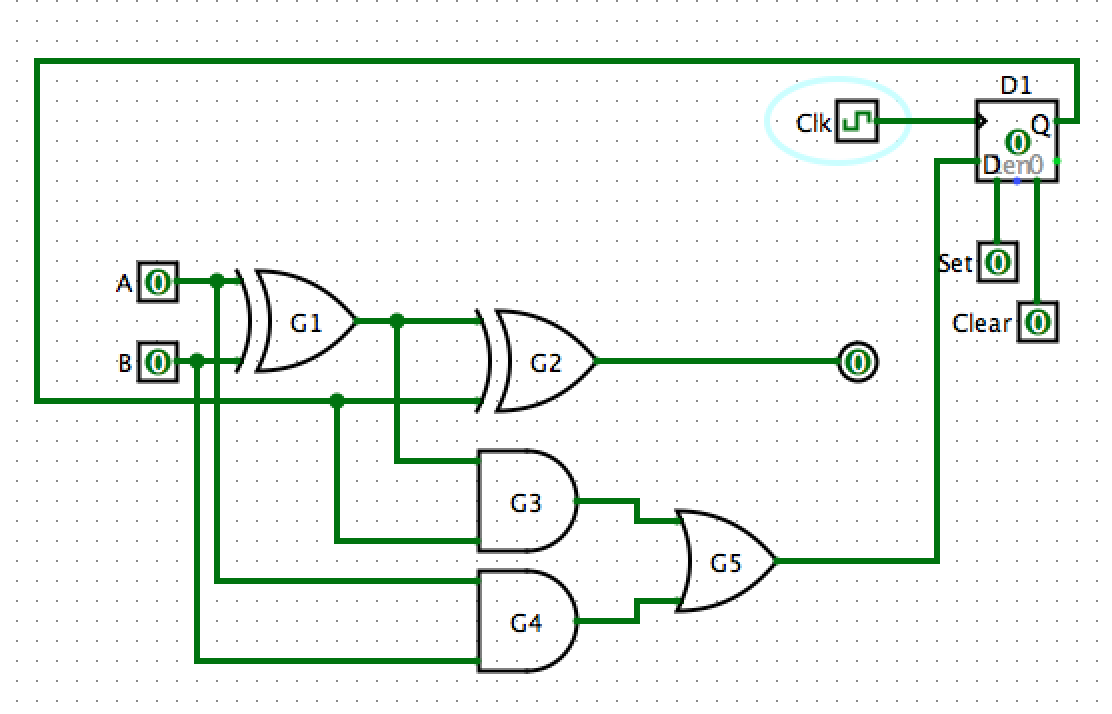
\includegraphics{sequential_carry_adder.png}
    \caption{circuit of a sequential carry adder}
\end{figure}

\VerbatimInput{sequential_carry_adder.txt}


\subsection{Binary Multiplier}
\begin{figure}[h]
    \centering
    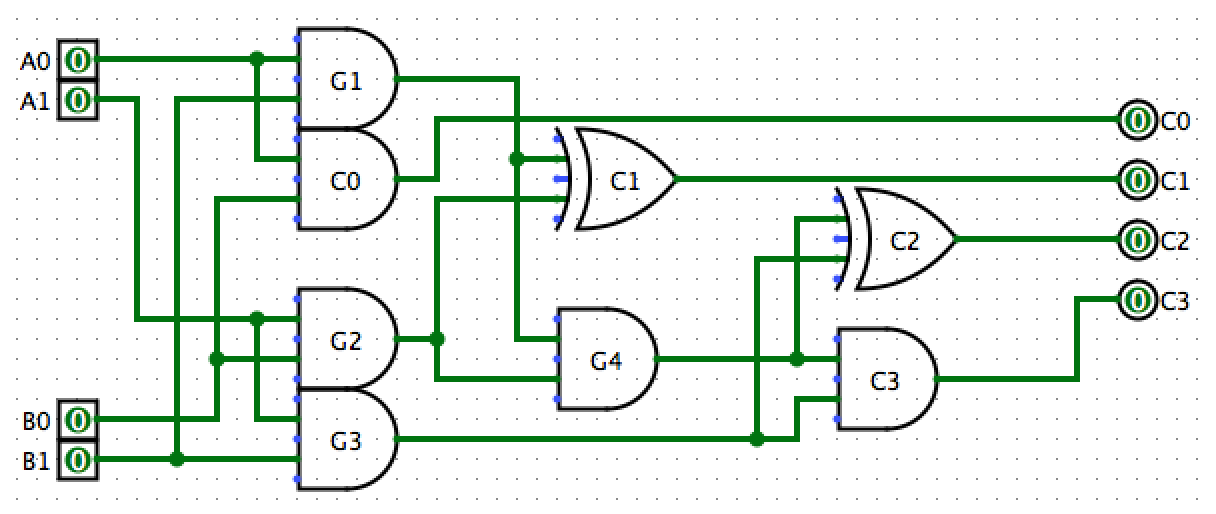
\includegraphics{bin_multiplier.png}
    \caption{circuit of a binary multiplier}
\end{figure}

\VerbatimInput{bin_multiplier.txt}




\end{document}



\end{document}